\documentclass[10pt,english]{article}
\usepackage[T1]{fontenc}
\usepackage[latin1]{inputenc}
\usepackage{fancyhdr}
\pagestyle{fancy}
\setlength\parskip{\medskipamount}
\setlength\parindent{0pt}
\usepackage{graphicx}
\IfFileExists{url.sty}{\usepackage{url}}
                      {\newcommand{\url}{\texttt}}

\makeatletter

\providecommand{\tabularnewline}{\\}

%%%%%%%%%%%%%%%%%%%%%%%%%%%%%% User specified LaTeX commands.
\usepackage{a4wide}
\usepackage{fancyhdr}

\usepackage{array}
\usepackage{graphicx}
\usepackage{setspace}

\lhead{KISS White Paper \\}

\usepackage{babel}

\usepackage{babel}
\makeatother
\begin{document}

%\date{\textbf{Revision/Date:} 01-00 - 2014-09-02}

\bigskip{}

%\begin{center}
\includegraphics[width=5cm]{figures/kiss.eps}
\rhead{ 
\includegraphics[width=2.cm]{figures/kiss.eps}}


\title{Kid Intereferogram Spectrometer Survey (KISS): a white paper}
\maketitle
\author{Authors here......}

%\offprints{A. Catalano - catalano@lpsc.in2p3.fr} %\email{catalano@lpsc.in2p3.fr} 

%\institute{Laboratoire de Physique Subatomique et de Cosmologie, 
%  CNRS/IN2P3, Universit\'e Joseph Fourier Grenoble I,
%  Institut National Polytechnique de Grenoble, 
%  53 rue des Martyrs, 38026 Grenoble Cedex, France 
%\and Institut N\'eel, CNRS, Universit\'e Joseph Fourier Grenoble I,
%  25 rue des Martyrs, Grenoble, France 
%\and IPAG: Institut de Plan\'etologie et d'Astrophysique d Grenoble, 
%  Universit\'e Joseph Fourier, Grenoble 1/CNRS-INSU, UMR 5274, 38041
 % Grenoble, France
%\date{Received XX, 2013; accepted XX, 2013}
%}
 \abstract
 {KISS is an low angular resolution spectrometer for continuum observations in millimeter and submillimeter wavelengths. Its wide spectral bandwidth, and highly multiplexed readout will enable to deeply observe cluster of galaxies via the Sunayev-Zel'dovich effect. The instrument consists of a Martin-Puplett interferometer optically coupled to a thousand LEKID array arranged in a dilution cryostat cooled at 100mK. The fast KID time response permits to perform high frequency interferograms (from 1 to 10 Hz) with a spectral resolution from 0.5 to 5 GHz strongly reducing the sky noise......}


\section{Science with KISS} \label{sec1}

\section{Science requirement} \label{sec1}

These science goals require measuring the sky brightness
at angular resolution of ten arc-min with a total field-of-view of few degrees in a high resolution wide spectral range. The galaxy cluster observations  do not require measuring the absolute spectrum of the sky background but a relative measurement between the source and the atmosphere is sufficient.  We keep the use of an internal blackbody calibrator to compare the sky signal as in COBE-FIRAS mission as an option; this option  will give us the access to CMB spectrum distortion measurements as a follow-up of COBE-FIRAS mission. The KISS proposed instrument is hence an spectrometer based on a Martin-Puplett fourier transform spectrometer with variable resolution (from 0.5GHz to 5GHz) using few thousands LEKIDs array cooled at 100 mK. The principal characteristics and the performance of the proposed KISS instrument are presented in Tab.\ref{tab:table_fin}


\subsection{Sensitivity}

The detectors mounted in the KISS instrument use the same technology developed with the NIKA and the NIKA2 instrument (cite several NIKA papers here). Considering the last NIKA observing campaigns, we expect to reach a sensitivity at the detector of the 20 mJy$\cdot \sqrt{s}$.

The fundamental limit to the instrument sensitivity is the atmospheric photon noise. In the Teide Observatory site this is expected to correspond to a photon-noise level per-pixel between 4 and 9 $\cdot$ 10$^{-17}$ W/$\sqrt{Hz}$ under a background of few tens of pW. 
Several laboratory measurements performed on NIKA arrays showed that the LEKIDs are already photon noise limited if we consider a realistic background for a ground based telescope as the 30m IRAM telescope. The noise equivalent temperature (NET) has been measured in laboratory adjusting continuously the sky simulator temperature between 50K and 300K. The results show a NET per pixel of about 1 mK/$\sqrt{Hz}$. Accounting for the optical chain transmission this corresponds to an optical noise equivalent power (NEP) of approximately 7x10$^{-17}$ W/$\sqrt{Hz}$ under a background of 20 pW minimum.
This level of sensitivity has been almost reached during the 2014 NIKA observing campaign.

\subsection{Angular resolution}
The KISS adopted solution is the use of a oversampled detector plane with respect to the diffraction spot size of about 10 arcmin. This gives us the sufficient amount of redundancy in the focal plane reconstruction. Starting from a typical NIKA rectangular pixel of 2 mm side, we preliminary optimised the focal plane with a final aperture ratio between 0.5 and 0.9 depending on the spectral frequency. The total useful projected field of view is approximately 3 x 3 deg$^{2}$.

\subsection{Spectral resolution}

The spectral resolution $\Delta \nu$ of a Martin-Puplett interferometer is :

\begin{equation}
\Delta \nu = \frac{c}{2 \Delta S}
\end{equation}

Where $c$ is the speed of light and $\Delta S$ is the maximum displacement of the roof mirror with respect to the other. 

In order to operate with a best spectral resolution of 0.5 GHz we need therefore to displace the roof mirror by  30 cm. 

\subsection{Scanning strategy}

Several kind of observation are required to efficiently reach the scientific targets:

\begin{itemize}


\item {\bfseries Tracked observations:} where the instrument tracks the source, i.e. it always observes the same position in the source referential.

\item {\bfseries On-The-Fly observations:} where the instrument continuously slews through the source with time to map it. 

\item {\bfseries Lissajous observations:} where the instrument performs Lissajous scan patterns to increase the mapping efficiency.

\end{itemize}

\begin{table*}[t!]
\begin{center}
\begin{tabular}{cc}
\hline \hline
{\bfseries Valid pixels} & 1000-2000  \\
{\bfseries Pixel size} [mm] & 2 \\
{\bfseries Dual polarization} &  yes \\
{\bfseries Angular size} ($F \lambda$) &  0.5-0.9 \\
{\bfseries Overall optical efficiency} [\%] &  30  \\
{\bfseries Field of view}~(deg) & 3  \\
{\bfseries FWHM}~(arcmin) &  10   \\
{\bfseries Band-pass}~(GHz) & 125-270    \\
{\bfseries Optical bandwidth}~($\delta \nu$ GHz) & 0.5-5    \\
{\bfseries Sensitivity at the detector}~(mJy$\cdot \sqrt{s}$) & 20   \\
{\bfseries Mapping speed}~(deg$^2$/mJy$^2$/hour) & 0.8   \\
\hline \hline
\end{tabular}
\end{center}
\caption{Characteristics and performance of the KISS instrument.}
\label{tab:table_fin}
\end{table*}



\subsection{Control of systematics}

We list in the following the principal source of systematic errors to be minimised:  

\begin{itemize}


\item {\bfseries Readout optimisation technique:} One of the most difficult challenges in operating with KIDs, is to convert the observed in phase (I(t)) and in quadrature (Q(t)) signal to absorbed optical power. This is a very different task with respect to the dissipative readout like thermal detectors (high impedance bolometer, TES, etc...). One possible solution is to perform a frequency sweep before starting each scan in the sky and to determine the centre of the resonance circle (I,Q) and calibrate the change of the phase ($\phi(f)$) as a function of frequency. The validity of this method depends directly on the stability of the atmosphere. Indeed, if the sky emission fluctuates during a scan, the resonance circle changes and therefore the responsivity of the detector changes. In order to improve the photometric reproducibility we developed a system to control the change of the signal by modulating the frequency on the local oscillator (by few kHz) synchronously to the FPGA in order to generate two tones one just below the resonant frequency of the detector. An average of 50 points is then performed in the FPGA acquiring data at the rate of 23.842 Hz. With this method it is possible to estimate the variation of the resonant frequency of the detectors $\Delta f_0(t)$, by projecting $(\Delta I(t), \Delta Q(t))$ along the gradient found as:
\begin{equation}
\Delta \hat{f_{0}}(t) = \frac{\left(\Delta I(t), \Delta Q(t)\right)\cdot\left(dI/df(t), dQ/df(t)\right)}{\left(dI/df(t), dQ/df(t)\right)^2}\cdot\delta f_{LO}
\label{eq:RFdIdQ}
\end{equation}

A detailed description of this method is given in \emph{Calvo et. al - 2013 }and \emph{Catalano et al - 2014}.

\item {\bfseries Field Of View (FOV) reconstruction : } In order to recover the pointing direction of each pixel, a focal plane reconstruction via planet scans is mandatory. We need to scan a bright astronomical source with the entire focal plane. Planets  as Jupiter and Mars has a small angular diameter compared to our beam and can be considered as a point source for the KISS observations. The position, width and the orientation of each KID can be determined by building a template of the low frequency part of the signal (mostly sky and electronic noise) using all detectors that are far from the source.

\begin{figure*}[b!]
\begin{center}
\includegraphics[width=13cm]{figures/dessin.eps} 
\end{center}
  \caption{Mechanical drawing of the KISS instrument together with the pointing system.}
\label{fig:dessin}
   \end{figure*} 

\item {\bfseries Atmosphere noise:}  Photometric calibration defines as well as possible the impact of systematic source of errors in the final sky maps. These sources of systematic errors come from \emph{external} uncertainties (calibration factors deduced from primary calibrator sources) or internal instrument uncertainties such as spectral response uncertainty, secondary beam fraction and opacity correction. In particular the opacity correction can be performed by using the KISS instrument as a tau-meter measuring the variation of the resonance frequencies of the detectors versus the airmass via elevation scans. This method has been successfully tested during the last NIKA observing campaigns. For more details see \emph{Catalano et al. - 2014}.

 
%We estimated that the overall calibration uncertainty for point sources on the final data at the map level is around 15~\% for 1.25~mm channel and 10~\% for 2.14~mm channel (see table \ref{table:perf}). This is based on the observed rms flux variation on a calibration source\cite{NIKA2014}. 


\item {\bfseries Sampling frequency:} As we mentioned before,  we need to perform interfererograms at a frequency faster then 1Hz In order to assure a low sky noise level. The fast KID time response permits to do it without any manifest loss of informations. The read out sampling frequency also has to follow this requirement. we proved that at least 100 points interferogram are needed in order to preserve all the spectral informations in the data, this means that the read out electronics has to work with a sampling frequency higher then 100 Hz.     

\end{itemize}

\section{Proposed KISS instrument} \label{sec1}

\begin{figure*}[b!]
\begin{center}
\includegraphics[width=12cm]{figures/optics.eps}
\end{center}
  \caption{Zemax simulation of the KISS optical path.}
\label{fig:optics}
   \end{figure*} 

\subsection{Pointing System}

The KISS pointing system will be assured by an altazimuth mount for supporting and rotating the instrument about two mutually perpendicular axes: the elevation axis must be rotated with a maximum amplitude of 60 degrees ($\pm 30$ with respect to the initial position pointing at 45 degrees as shown in Fig \ref{fig:dessin}) because of cryostat limitations. The two-axis drive systems, to track equatorial motion, is performed by a .......
 {\bfseries Explain the rotation degrees of freedom and the way to control it here.....}

\subsection{Martin-Puplett Interferometer}

The KISS Martin-Puplett interferometer must satisfy two main requirements: first, it has to guarantee performance good enough for all the optical fields from 0 to 3 degrees. Second, it must be able to perform continuously 30cm path interferograms at a frequency higher than 1 Hz. These two requirements  have been studied and a preliminary drawing is presented in Fig \ref{fig:optics} for the optics and in Fig. ({\bfseries mechanical drawing from Monica}).  One of the two roof mirrors is moved by a mechanical-bearing direct-drive linear stage.

The manufacturing of the mechanical piece will be fully developed, executed and tested between the LPSC and the N�el institute  in Grenoble.  


\subsection{Cryogenic system}

The KISS cryostat will be the one used for the NIKA prototype instrument. It consists of a 4~K cryocooler and a closed-cycle $^3$He - $^4$He dilution. All the system can be easily operated and controlled from a remote station with very few a local interventions such as the switching on and off of the pulse tube, and the refilling of the nitrogen carbon trap (used to prevent impurities into the mixture circuit).  The detectors are sensitive to magnetic fields due to the Earth and all the instrumentation present on site. In order to reduce these potential noise sources, two magnetic shields have been added: mu-metal at 300~K and a superconducting lead screen on the 4K stage. 

\subsection{Optics} 

KISS optical elements consist of 2 conical mirrors (1m and 0.3m diameter), 5 polyethylene and quartzes lenses inside the MP interferometer and the cryostat, several pass-band and low-pass metal mesh filters to define the shape the width and the position of the KISS final bandpass. All the lenses are telecentric that is each point of the detector plane is illuminated with the same aperture with the chief ray perpendicular to the surface. The Zemax optical simulation with preliminary optimisation is presented in Fig. \ref{fig:optics}

{\bfseries Maybe here we should present the KISS bandpass (the convolution of the two channels of NIKA instrument) compared to the atmospheric emission model with different vapour contents......}

\subsection{Focal plane and detectors}

The adopted solution for the KISS instrument uses dual-polarization LEKIDs using a Hilbert pattern inductor (Roesch 2012). LEKID array will fully sample the field-of-view of 3 degrees using from 1000 to 2000 LEKIDs detectors arranged in a single array.  It comprises four readout lines and the pixels, for a fully
filled focal plane diameter of 80 mm. The detectors are realised from a single Aluminium
(thickness from 12 to 25 nm) film on a 100 mm Silicon wafer. An Anti-Reflecting
treatment is applied by micro-machining or dicing to the back of the wafer to improve
the spectral response flatness of the LEKID.
The first prototypes of the array have been already fabricated and tested in Grenoble.  The exact design and the fabrication details are entirely derived from the NIKA developments.


\begin{figure*}[b!]
\begin{center}
\includegraphics[width=7.5cm]{figures/miroir_cryo.eps} 
\includegraphics[width=6.77cm]{figures/array.eps} 
\end{center}
  \caption{Left: Dilution cryostat working in the 30m IRAM receiver cabin. Right: prototype of 1900 pixel LEKIDs array.}
\label{fig:kid_cryo}
   \end{figure*} 



\subsection{Readout electronics, data acquisition and pipeline}

The warm electronics for KISS is the NIKEL system described in more detail
by \emph{Bourrion et al. - 2012} and successfully used in NIKA  and preliminary in NIKA2 instruments. 
NIKEL allows a multiplexed readout of up to 400 channels/pixels over 500
MHz bandwidth. It generates the modulated signal needed by the RF synthesizers, averages the I,Q data down to the final rate (maximum permitted rate equal to 1 kHz) and diffuses them by
UDP (User Datagram Protocol) packets over a local network to the acquisition computers.
\\
\\
We already developed a dedicated reduction pipeline to calibrate, filter and process data onto sky maps for the NIKA instrument. The principal steps of the processing (raw data creation, flagging bad detectors, data filtering, calibration procedure, noise decorrelation and map making) will be unchanged. 


%We describe briefly the working principle of NIKEL:  6 separate Field Programmable Gate Arrays (FPGAs), are coupled to a Digital to Analog Converter; they can generate a comb of frequencies (up to 400 tones) each over a 500~MHz bandwidth each set to the resonant frequency of a LEKID in the array. The comb is then up converted by mixing with a local oscillator carrier at the appropriate frequency. The resulting signal is fed into the cryostat using a single coaxial line, and excites each resonator. On the output line, one cryogenic low noise amplifier boosts the signal of each read out tone, which then is down-converted to the base band and is acquired by an Analog to Digital Converter (ADC). The output tones are compared to a copy of the input tones kept as a reference, so that for each pixel it is possible to measure the component of the signal that is in phase (I) and in quadrature (Q) with respect to the reference. Five of the FPGAs generate 80 tones each over a 100~MHz band, using five associated DACs. The sixth FPGA acts as a central unit that combines the signal of the other units, appropriately shifting and filtering the different 100~MHz sub-bands to finally cover the whole 500~MHz available for the frequency comb used to excite the detectors. An analogous,
%but reversed, process is then applied to the signal acquired by the ADC of the board, which is once again split in 5 different sub-bands treated separately.

\section{Complementarity with other experiments}

--  SUPERSPEC
\\
\\
--  MILLIMETRON
\\
\\
--  OLIMPO ??? 
\\
\\
--  OTHERS ???


\bibliographystyle{aa}
\bibliography{cata2}


\end{document}
